\chapter{Theoretical Background}\label{ch_theoretical_background}

The related work survey identified that existing tools operate on individual optimisation dimensions - tile data pruning, encoding, or style cleanup - but none composes them into a joint pipeline, and none draws systematically on compiler or database optimisation theory.
Building such a pipeline requires foundations from several fields: the map rendering architecture that defines what is being optimised, the compiler techniques whose analogues drive the expression-level passes, the query optimisation concepts that inform filter rewriting and predicate reordering, and the columnar encoding strategies that underpin the data-level passes.

This chapter introduces these foundations in the order in which the optimiser consumes them.
\cref{sec_map_rendering_approaches} describes the map rendering process and its resource pipeline.
\cref{sec_compiler_optimizations} surveys compiler optimisation techniques - peephole rewriting, constant folding, and fixpoint iteration - whose analogues are applied to style expressions.
\cref{sec_query_optimizations} presents query optimisation concepts - predicate pushdown and selectivity estimation - used for filter rewriting and reordering.
\cref{sec_data_encoding} covers the columnar encoding and compression schemes employed at the tile level.
\cref{sec_multi_objective_optimizations} discusses multi-objective optimisation, \cref{sec_benchmarking} covers benchmarking methodology, and \cref{sec_problem_statement} formalises the optimisation problem that \cref{ch_methods} addresses.

\section{Map Rendering Approaches}\label{sec_map_rendering_approaches}

When building a slippy map (i.e.\ a map with the modern pan, zoom, rotation, and interaction capabilities), the technology stack is fairly simple.

A user interacts with an input device (mouse, touch, keyboard) to control the map view.
The map view is rendered using one of the following approaches:

\begin{itemize}
\item \begin{sloppypar}\textbf{SVG} is a vector graphics format that can be used to render maps as shown by the ID Editor~\cite{OpenstreetmapID2026} or Leaflet~\cite{LeafletOpensourceJavaScript}.
Using SVGs means one is limited to a 2D rendering approach due to not having a camera.\end{sloppypar}

\item \textbf{Canvas 2D} is the HTML5 \texttt{<canvas>} immediate-mode drawing API.
OpenLayers~\cite{OpenLayers} uses Canvas~2D as its primary renderer, rasterising vector features on the CPU rather than submitting them to the GPU.
This avoids the complexity of GPU pipeline management and shader compilation, but rendering throughput is CPU-bound and does not benefit from hardware-accelerated geometry processing.
Like SVG, Canvas~2D is limited to 2D views without pitch or rotation.

\item \begin{sloppypar}\textbf{Low-level 3D Graphics APIs} like WebGL~\cite{WebGLLowLevel3D2011}, WebGPU~\cite{WebGPU}, OpenGL~\cite{OpenGL4Reference}, Metal~\cite{incMetalOverview}, Vulkan~\cite{HomeVulkanCross}, DirectX~\cite{DirectXSpecs}, etc.\ for rendering 3D graphics as shown by mapbox~\cite{MapboxMapsNavigation}, maplibre~\cite{maplibreMapLibre}, deck.gl~\cite{HomeDeckgl}, here~\cite{HERETechnologiesWorlds} and many more.
This allows a more complex 3D-based rendering with pitch, yaw, and roll.
Due to having better hardware access, these APIs can render more complex scenes with better performance.\end{sloppypar}
\end{itemize}

Due to the more advanced features and mostly better performance, this research focuses exclusively on renderers based on open-source 3D graphics APIs.
While these renderers are powerful, they require data to be preprocessed and optimized specifically for rendering.
As a result, they cannot directly render high-level primitives such as shapes (polygons, lines, points), text, or images.
Instead, they operate on lower-level graphics primitives such as textures, triangles, and quads.

These low-level graphics building blocks are linked to map data through sprites, fonts, and styles, which are then interpreted by a rendering engine.

\newpage
As a lower-level representation layer for displaying map content, the following components are required, as shown in \cref{fig:basic-arch}:

\begin{itemize}
\item styles define the visual appearance of the map and reference the other required resources,
\item tiles provide the geometry (points, lines, polygons) and associated attributes (for example, building heights) displayed on the map,
\item sprites supply the icons shown on the map,
\item fonts provide the glyphs used to render text labels.
\item sometimes, additional assets such as 3D geometry models or terrain is used
\end{itemize}

\begin{figure}[h]
\centering
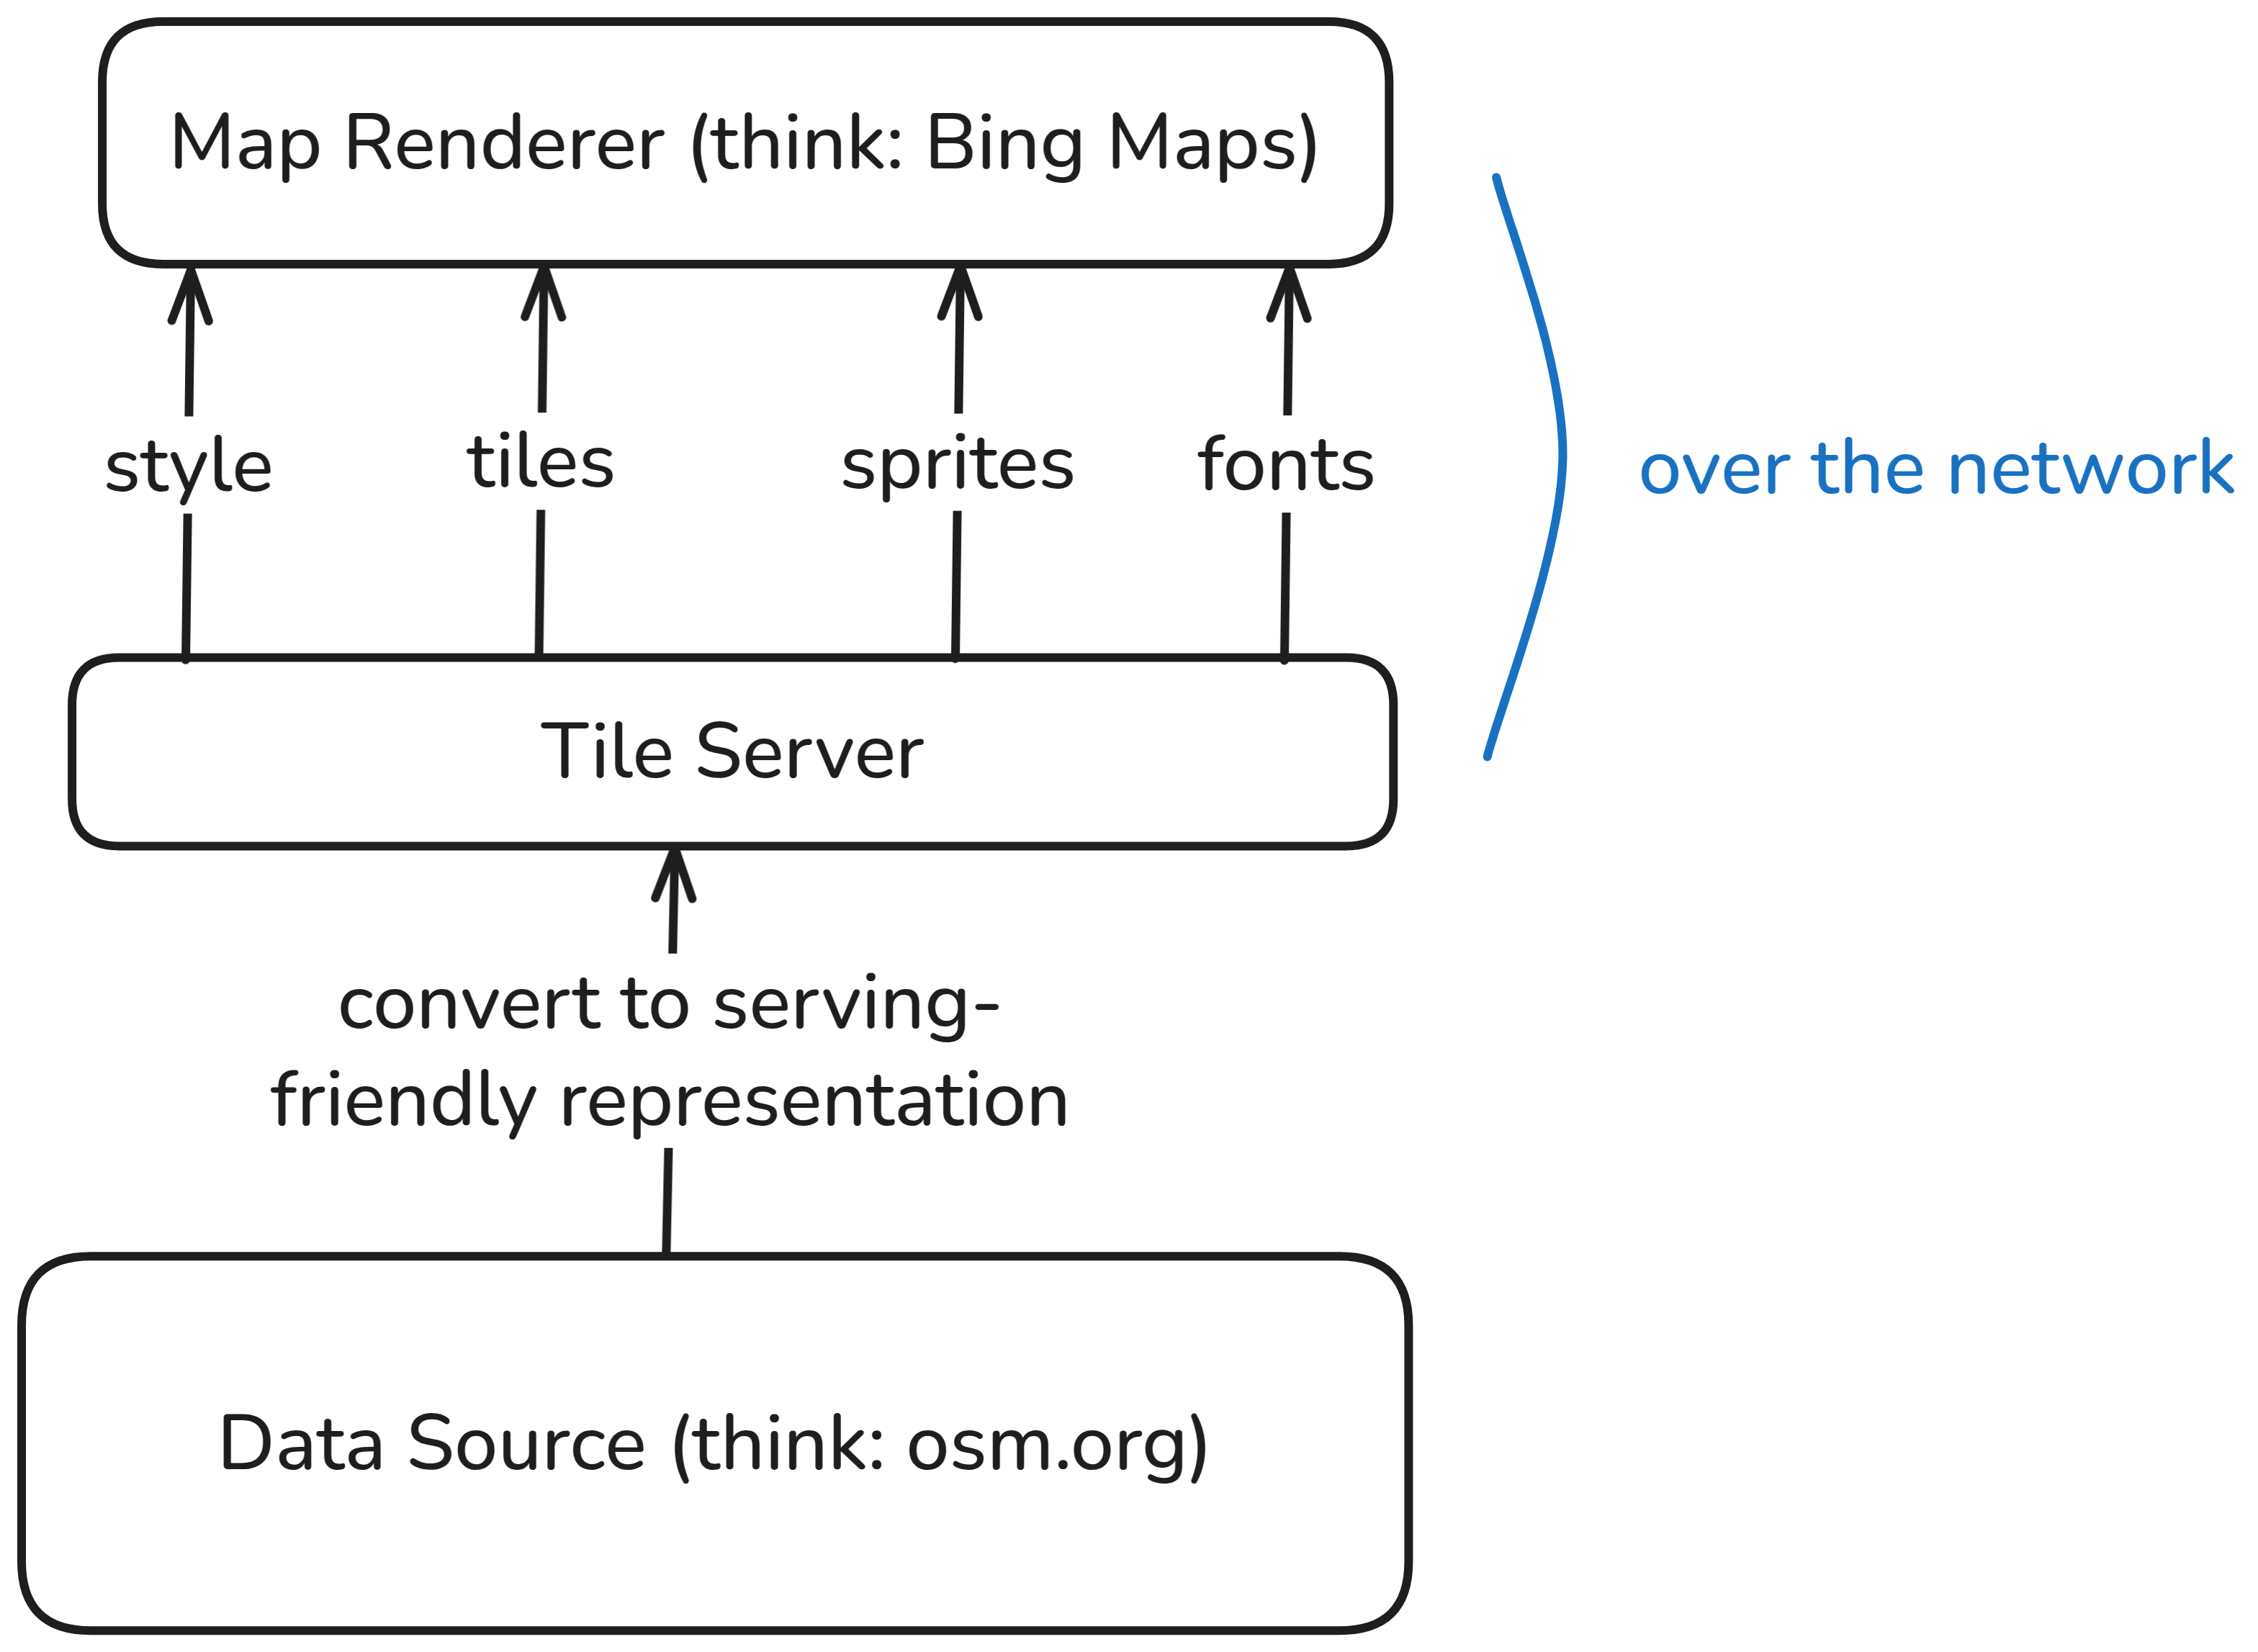
\includegraphics[width=0.5\linewidth]{figures/basic-architecture.png}
\caption{Basic building blocks of a map rendering stack. Data is taken from a data source, converted into a simplified format (for example a spatial index), and served to a client. The visual appearance is defined by a style and supported by fonts and sprites for text and icons.}
\label{fig:basic-arch}
\end{figure}

There are several approaches to delivering client-side rendered vector maps.

Styles, sprites, and fonts are typically served from a file server or \ac{CDN} and require little processing.
In some cases, parts of these resources may be generated dynamically - for example, to support complex text shaping for Arabic, Hebrew, Indic, or Japanese scripts as described by Wipfli~\cite{ComplexTextPlugin} for MapLibre or Lengyel~\cite{https://terathon.com/blog/decade-slug.html} for SLUG.
This processing currently usually handled ahead of time on the server-side.

Tiles, by contrast, can be stored and accessed using three major approaches:

\begin{itemize}
\item
    \textbf{Dynamic}:
    Store geospatial data in a database (for example, PostGIS) and use a tile server to generate and serve tiles on demand.
\item
    \textbf{Client-driven}:
    Store encoded tiles as a single file in a blob store using a format that includes an internal tile index (for example, PMTiles or VersaTiles).
    Clients retrieve tiles using multiple HTTP requests with appropriate Range headers to locate the required data.
\item
    \textbf{Semi-static}:
    Store encoded tiles in a database file on disk (for example, SQLite) and use a tile server to extract and serve tiles to clients.
\end{itemize}

Dynamic data sources can be updated frequently by applying incremental diffs, whereas the other approaches typically require a full rebuild when the underlying data changes.
At larger scales, in-memory caching of tiles via regional or \ac{CDN}-style infrastructure - combined with fallback to runtime-dynamic data - is essential for performance.

Although all of these resources can be optimized, tiles are usually the most critical due to their continuous streaming nature as a user moves the map thus higher data volume.
All other resources depend on locale sligtly (for example loading different unicode ranges or fonts), but are generally only handled one time.

Real-world observations support this:
the performance of highly optimized systems such as Microsoft Bing Maps differs significantly from less optimized deployments, such as basemap.de.

The following sections examine each resource in detail, focusing on the performance characteristics and optimizations strategies relevant to this work:

\subsection{Fonts}

Fonts can be client rendered from a font file.
This requires shipping a font renderer to the client, as neither native nor web targets have for example Harfbuzz as a feature.
This also means that for some fonts up to \qty{30}{\mega\byte} of font data needs to be transferred.

For interactive use cases, this is prohibitive as the time to download this would be longer than acceptable.
Some fonts need this shaping as they need to connect neigboring characters neatly, but Latin fonts do usually not.
For latin-like characters, there is usually a clear 1:1 relationship between the Unicode code point and a rendered character.

This is why a simpler way exists:
Cutting fonts up into Unicode slices (\texttt{start..end}) and serving only the ranges that are needed to the client.
This cutting of fonts has the implicit advantage of pruning the space of possible font data to just the data that is needed to render the map.

Common open-source renderers like MapLibre or source-available renderers like Mapbox do this by shipping pre-rasterised glyph ranges as \acp{PBF} encoded \acp{SDF}, indexed by Unicode range (e.g.\ \texttt{0-255.pbf}, \texttt{256-511.pbf}).

\subsection{Sprites}

Sprites in computer graphics are a fairly solved problem.
To avoid having to request hundreds to thousands of small files or to have to render SVGs on a client, this work is shifted to the server and the server delivers sprite sheets.
This allows efficient GPU Sprite instancing.

Common open-source renderers like maplibre or source available renderers like mapbox do this by shipping both

\begin{itemize}
\item plain PNG or \acs{SDF}-PNG~\cite{greenImprovedAlphatestedMagnification2007} sprite sheets, in combination with
\item a lookup table of where on the sprite sheet each sprite is located, whether the sprite is a \ac{SDF}, and whether there are regions of the sprite that can be stretched to account for placing text inside the sprite.
\end{itemize}

\subsection{Tiles}\label{sec_tiles}

Tiles are the primary data delivery mechanism for interactive web maps.
Rather than transferring the entire dataset to the client, the map is partitioned into a regular grid of square tiles at discrete zoom levels following the widely adopted XYZ tiling scheme.
At zoom level~$z$, the world is subdivided into $2^z \times 2^z$ tiles, each identified by its column~$x$, row~$y$, and zoom level~$z$.
Lower zoom levels cover large geographic areas with simplified geometry; higher zoom levels cover smaller areas with greater detail.
The client requests only the tiles intersecting the current viewport, and as the user pans or zooms, new tiles are fetched while old ones are discarded or cached.
When a client requests a tile at a zoom level beyond the source's maximum, the renderer \emph{overzooms}: it upscales the nearest available tile from the source's highest available zoom to fill the viewport.
The \emph{layers} sourced from that tile remain rendered at the overzoomed level even though no new tile is fetched, which means that a layer's effective visibility at a given camera zoom cannot be determined from filter or data bounds alone - it is a function of both the layer's filter and the source's \texttt{maxzoom}.
This observation has direct consequences for any optimiser that rewrites zoom bounds, and is revisited in \cref{ch_methods}.
\Cref{lst:overzoom} shows the implementation: when overzoom parameters are present, the worker source substitutes a sliced version of the source's \texttt{maxzoom} tile.
The slicing function rescales geometry coordinates into the target tile's coordinate space and clips to the tile extent, producing a synthetic tile from the nearest available data.

\begin{lstlisting}[language=TypeScript,caption={MapLibre GL-JS overzoom implementation (\texttt{src/source/vector\_tile\_overzoomed.ts:87--125})},label=lst:overzoom]
export function sliceVectorTileLayer(sourceLayer: VectorTileLayerLike, maxZoomTileID: CanonicalTileID, targetTileID: CanonicalTileID): VectorTileLayerOverzoomed {
    const {extent} = sourceLayer;
    const dz = targetTileID.z - maxZoomTileID.z;
    const scale = Math.pow(2, dz);

    // Calculate the target tile's position within the source tile in target coordinate space
    // This ensures all tiles share the same coordinate system
    const offsetX = (targetTileID.x - maxZoomTileID.x * scale) * extent;
    const offsetY = (targetTileID.y - maxZoomTileID.y * scale) * extent;

    const featureWrappers: VectorTileFeatureOverzoomed[] = [];
    for (let index = 0; index < sourceLayer.length; index++) {
        const feature: VectorTileFeatureLike = sourceLayer.feature(index);
        let geometry = feature.loadGeometry();

        // Transform all coordinates to target tile space
        for (const ring of geometry) {
            for (const point of ring) {
                point.x = point.x * scale - offsetX;
                point.y = point.y * scale - offsetY;
            }
        }

        const buffer = 128;
        geometry = clipGeometry(geometry, feature.type, -buffer, -buffer, extent + buffer, extent + buffer);
        if (geometry.length === 0) {
            continue;
        }

        featureWrappers.push(new VectorTileFeatureOverzoomed(
        feature.type,
        geometry,
        feature.properties,
        feature.id,
        extent
        ));
    }
    return new VectorTileLayerOverzoomed(featureWrappers, sourceLayer.name, extent);
}
\end{lstlisting}

No symmetric \enquote{underzoom} behaviour exists: if a source has no tile at a zoom lower than \texttt{minzoom}, the layer is simply not rendered there.

A \emph{vector tile} encodes map data in a compact binary format rather than as a pre-rendered image.
Each tile is organised into \emph{source layers} (for example, roads, buildings, water), and each source layer contains a set of \emph{features}.
A feature consists of
\begin{itemize}
    \item geometry (point, linestring, or polygon encoded as integer coordinates relative to the tile's extent)
    \item optionally, a set of key--value \emph{properties} (for example, \texttt{class=motorway} or \texttt{name=Main~Street})
    \item optionally, a set of ids
    \item metadata like extent
\end{itemize}

The following formats are used for encoding and transferring vector map data to the client:

\begin{itemize}
    \item \textbf{GeoJSON}~\cite{rfc7946} is a JSON-based geospatial interchange format.
    Its human-readable structure makes it useful for debugging and small overlays, but its verbosity - text-encoded coordinates and repeated property keys per feature - makes it impractical for the continuous tile streaming required by interactive map renderers.

    \item \textbf{\acf{MVT}}~\cite{MapboxVectorTileSpec} is the dominant vector tile format, adopted as a \emph{de~facto} standard across open-source map renderers including MapLibre.
    It uses Protocol Buffers~\cite{ProtocolBuffers} as its wire format and stores features in a \emph{row-oriented} layout: each feature carries its own list of property tags encoded as alternating key and value indices into per-layer string and value tables.
    Geometry is encoded as a sequence of \texttt{MoveTo}, \texttt{LineTo}, and \texttt{ClosePath} commands with delta-encoded integer coordinates relative to the tile extent (typically 4096 units per tile edge).
    The row-oriented layout means that accessing a single property column requires parsing past all other properties of the same feature, and that compression operates on the interleaved byte stream rather than on homogeneous data columns.

    \item \begin{sloppypar}\textbf{\acf{MLT}} is a columnar vector tile format proposed by Tremmel et~al.~\cite{tremmelMapLibreTileNext2025}.
    Instead of the row-major key--value-pair layout of \ac{MVT}, \ac{MLT} stores each property as an independent column with type-specific encoding.
    This columnar layout enables per-column compression strategies - for example, dictionary encoding for low-cardinality string columns, delta encoding for monotonically increasing integers, or run-length encoding for repeated values - and eliminates the per-feature tag overhead of the protobuf encoding.
    Tremmel et~al.\ report 2--6$\times$ tile size reductions over \ac{MVT} depending on data characteristics.\end{sloppypar}

    \item \textbf{Analysis-focused formats} such as FlatGeoBuf, GeoParquet, and GeoArrow are optimised for analytical queries (filtering, aggregation, joins) rather than tile-based rendering.
    They support random access and columnar scans but do not follow the tiled spatial access pattern required by interactive map renderers and are therefore not considered further in this work.

    \item \textbf{Raster tiles} deliver pre-rendered images (PNG, JPEG, WebP) rather than vector geometry.
    They require no client-side rendering logic but cannot be restyled, rotated at arbitrary angles, or queried interactively, as the visual representation is fixed at generation time.
\end{itemize}

Beyond the choice of tile format, a number of transfer-layer optimizationss can improve delivery performance: utilising the approximately \qty{14}{\kilo\byte} TCP slow-start window as discussed by Nathaniel~\cite{WhyYourWebsite}, edge caching~\cite{BestPracticesMap}, or HTTP/2 multiplexing.
Since \ac{MVT} is the established baseline and \ac{MLT} aims to improve upon it, this thesis evaluates both formats and uses the transition from \ac{MVT} to \ac{MLT} as one of its data-level optimizations strategies.

\subsection{Styles}\label{sec_styles}

A map style defines the complete visual appearance of a map: which data is shown, how it is coloured, sized, and labelled, and at which zoom levels each element appears.
Three architectural approaches to map styling have been established:

\begin{itemize}
    \item \textbf{Server-side declarative} styles, such as MapCSS, define rendering rules on the server.
    The server evaluates the style against the data and produces pre-rendered raster tiles that the client displays without further interpretation.
    This simplifies the client but prevents client-side restyling and limits interactivity.

    \item \begin{sloppypar}\textbf{Client-side declarative} styles, as used by MapLibre~\cite{maplibreMapLibre} and Mapbox~\cite{MapboxMapsNavigation}, transmit a machine-readable style document to the client, which interprets the style at render time.
    This enables dynamic restyling, data-driven visualisation, and interactive features such as hover effects and click queries without regenerating tiles.\end{sloppypar}

    \item \textbf{Callback-based} styling, as proposed by Gleo~\cite{ortegaGleoWebGLMap}, replaces declarative rules with imperative callbacks that the application registers with the renderer.
    This offers maximum flexibility but makes static analysis and automatic optimizations impossible, since the styling logic is opaque to the rendering engine.
\end{itemize}

This thesis focuses on client-side declarative styles, specifically the MapLibre style specification, as it is the most widely adopted approach in open-source map rendering and - its declarative nature makes it amenable to static analysis and automatic optimizations.

The MapLibre style specification~\cite{MapLibreStyleSpec} defines a map's appearance as a JSON document with the following key components:

\begin{itemize}
    \item \textbf{Sources} declare where tile data comes from (a tile server URL, an MBTiles file, or inline GeoJSON) and at which zoom levels tiles are available (\texttt{minzoom}, \texttt{maxzoom}).

    \item \textbf{Layers} are the central rendering unit.
    Each layer references a source and a \emph{source-layer} within that source, specifies a \emph{type} - one of \texttt{fill}, \texttt{line}, \texttt{circle}, \texttt{symbol}, \texttt{fill-extrusion}, \texttt{raster}, \texttt{background}, or \texttt{hillshade} - and carries a set of paint and layout properties that control its appearance.
    Layers are drawn in declaration order from bottom to top.

    \item \textbf{Filters} are boolean expressions attached to layers that select which features from the source-layer are rendered.
    A feature is drawn by a layer only if the layer's filter evaluates to \texttt{true} for that feature's properties and geometry type.

    \item \textbf{Paint and layout properties} control the visual appearance and placement of rendered features.
    Paint properties (colours, opacities, widths) can be changed without triggering a re-layout; layout properties (text anchoring, icon rotation, symbol spacing) affect feature placement and require re-evaluation when modified.

    \item \textbf{Metadata bounds} (\texttt{minzoom}, \texttt{maxzoom}) restrict the zoom range at which a layer is active, allowing the renderer to skip entire layers outside their visible range without evaluating their filters.
    \Cref{lst:ishidden} shows the implementation: the method checks the layer's zoom bounds and evaluated visibility in a single guard, and is called at both tile-parse time (the worker skips bucket creation) and draw-call time (the painter skips rendering).
    Tight \texttt{minzoom}/\texttt{maxzoom} bounds therefore eliminate work at two stages of the pipeline before any filter evaluation or geometry decoding occurs.

\begin{lstlisting}[language=TypeScript,caption={MapLibre GL-JS \texttt{isHidden} method and its call sites (\texttt{src/style/style\_layer.ts:328--332}, \texttt{src/source/worker\_tile.ts:111}, \texttt{src/render/painter.ts:658--659})},label=lst:ishidden]
// src/style/style_layer.ts:328-332
isHidden(zoom: number = this.minzoom, roundMinZoom: boolean = false) {
    if (this.minzoom && zoom < (roundMinZoom ? Math.floor(this.minzoom) : this.minzoom)) return true;
    if (this.maxzoom && zoom >= this.maxzoom) return true;
    return this._evaluatedVisibility === 'none';
}

// src/source/worker_tile.ts:111 -- worker skips bucket creation
if (layer.isHidden(this.zoom, true)) continue;

// src/render/painter.ts:658-659 -- painter skips draw calls
renderLayer(painter, tileManager, layer, coords, renderOptions) {
    if (layer.isHidden(this.transform.zoom)) return;
    // ...dispatches to draw.fill, draw.line, draw.symbol, etc.
}
\end{lstlisting}

\end{itemize}

Filters and properties can be specified as literal constants, as \emph{zoom-dependent} expressions (varying with the camera zoom level via \texttt{interpolate} or \texttt{step} ramps), as \emph{data-driven} expressions (varying per feature based on property values via \texttt{match}, \texttt{case}, or \texttt{get} operators), or as a combination of both.
The resulting expression trees can be deeply nested and may contain redundant or unreachable branches - characteristics that make them amenable to the same kinds of simplification and optimizations techniques used in compilers and database query planners.

\Cref{lst:worker_pipeline} shows how these components interact in practice: MapLibre's worker thread parses a tile by iterating source layers, collecting features, checking \texttt{isHidden}, recalculating layer expressions at the current zoom, and populating buckets (which runs the filter and builds vertex data).
Every optimisation in \cref{ch_methods} maps to a step in this pipeline.

\begin{lstlisting}[language=TypeScript,caption={MapLibre GL-JS worker tile processing pipeline (\texttt{src/source/worker\_tile.ts:85--127})},label=lst:worker_pipeline]
// src/source/worker_tile.ts:85-127 -- WorkerTile.parse()
const layerFamilies = layerIndex.familiesBySource[this.source];
for (const sourceLayerId in layerFamilies) {
    const sourceLayer = data.layers[sourceLayerId];
    if (!sourceLayer) continue;

    const features = [];
    for (let index = 0; index < sourceLayer.length; index++) {
        const feature = sourceLayer.feature(index);
        const id = featureIndex.getId(feature, sourceLayerId);
        features.push({feature, id, index, sourceLayerIndex});
    }

    for (const family of layerFamilies[sourceLayerId]) {
        const layer = family[0];
        if (layer.isHidden(this.zoom, true)) continue;       // metadata skip
        recalculateLayers(family, this.zoom, availableImages); // eval at zoom

        const bucket = layer.createBucket({/*...*/});
        bucket.populate(features, options, this.tileID.canonical); // filter + encode
    }
}
\end{lstlisting}

\section{Compiler Optimisation Techniques}\label{sec_compiler_optimizations}

The style expressions used by map renderers such as MapLibre are, in essence, small programs: they contain conditionals (\texttt{case}, \texttt{match}), boolean operators (\texttt{all}, \texttt{any}), arithmetic, and data access (\texttt{get}, \texttt{has}).
Optimising these expressions draws directly on techniques developed over decades in compiler construction~\cite{ahoCompilersPrinciplesTechniques2006}.
This section introduces the foundational concepts applied in \cref{ch_methods}.

\subsection{Peephole Optimisation}

\begin{sloppypar}
A \emph{peephole optimiser} examines a small, fixed-size window of code (the \enquote{peephole}) and applies local pattern-matching rewrites that replace instruction sequences with shorter or faster equivalents~\cite{davidsonImprovingInstructionSelection1984}.
Each rewrite rule is independent: it matches a local pattern and emits a replacement, without requiring knowledge of the surrounding program.
The simplicity of individual rules is offset by their composition through repeated application - many small, local improvements accumulate into significant global optimizations.
\end{sloppypar}

Peephole optimisers are classified by the level at which they operate.
\emph{Machine-level} peephole optimisers replace instruction sequences (e.g., replacing a multiply by a power of two with a shift).
\emph{\ac{IR}-level} peephole optimisers apply algebraic simplifications, identity eliminations, and strength reductions to expression trees.
In the context of style expressions, the peephole window corresponds to a single expression node and its immediate children.
A post-order visitor walks the expression tree and attempts to apply each rule at every node, producing a locally simplified tree.

\subsection{Constant Folding and Propagation}

\emph{Constant folding} evaluates expressions whose operands are all compile-time constants, replacing the expression with its result~\cite{ahoCompilersPrinciplesTechniques2006}.
For example, the expression $3 + 5$ is replaced by $8$.
In a style context, a comparison such as \texttt{["==",~2,~3]} can be evaluated at optimizations time and replaced by \texttt{false}.

\emph{Constant propagation} extends this idea by tracking the known values of variables through the program's control flow and substituting them at their use sites.
If a variable is assigned a constant, all subsequent references to that variable can be replaced by the constant, potentially enabling further constant folding at the use sites.

A more powerful variant, \acf{SCCP}, combines constant propagation with dead branch analysis in a single pass: it simultaneously determines which values are constant \emph{and} which branches are reachable, enabling the discovery of constants that are only visible when unreachable code is ignored~\cite{wegmanConstantPropagationConditional1991}.

\subsection{Dead Code Elimination}

\acf{DCE} removes program statements whose results are never used or whose control-flow paths are unreachable~\cite{ahoCompilersPrinciplesTechniques2006}.
Two common forms are:

\begin{itemize}
    \item \emph{Unreachable code elimination}: removing code that can never be executed (e.g., code after a guaranteed return, or branches guarded by a statically false condition).
    \item \emph{Dead store elimination}: removing assignments to variables that are never subsequently read.
\end{itemize}

In the map-style domain, dead code elimination corresponds to removing style layers that can never produce visible output - because their filter is unsatisfiable, their geometry type does not match the data, or their paint properties render them invisible (e.g., zero opacity at all zoom levels).

\subsection{Algebraic Simplification}

\emph{Algebraic simplification} applies mathematical identities to reduce expression complexity without changing semantics~\cite{ahoCompilersPrinciplesTechniques2006}.
Common algebraic rules include:

\begin{itemize}
    \item \emph{Identity elements}: $x \land \mathit{true} = x$,\quad $x \lor \mathit{false} = x$,\quad $x + 0 = x$,\quad $x \cdot 1 = x$.
    \item \emph{Annihilation}: $x \land \mathit{false} = \mathit{false}$,\quad $x \lor \mathit{true} = \mathit{true}$,\quad $x \cdot 0 = 0$.
    \item \emph{De~Morgan's laws}: $\lnot (a \land b) = \lnot a \lor \lnot b$ and $\lnot (a \lor b) = \lnot a \land \lnot b$.
    \item \emph{Idempotence}: $x \land x = x$,\quad $x \lor x = x$.
    \item \emph{Absorption}: $x \land (x \lor y) = x$,\quad $x \lor (x \land y) = x$.
\end{itemize}

For style expressions, these rules simplify boolean filter expressions.
A filter \texttt{["all", ["all", a, b], c]} is flattened to \texttt{["all", a, b, c]} by the associativity of conjunction, and \texttt{["all", true, x]} is simplified to~\texttt{x} by identity elimination.

\subsection{Fixpoint Iteration}\label{sub_fixpoint}

Individual peephole rules may expose further optimizations opportunities: constant folding a subexpression may create a new constant parent, which in turn enables dead branch elimination.
A single traversal is therefore generally insufficient.

\begin{sloppypar}
\emph{Fixpoint iteration} addresses this by applying the entire rule set repeatedly until no rule fires - that is, until the expression reaches a \emph{fixpoint} at which no further rewrites apply.
For a monotone transformation $f$ on a finite domain, the sequence $x,\, f(x),\, f(f(x)),\, \ldots$ is guaranteed to converge~\cite{ahoCompilersPrinciplesTechniques2006}.
In practice, convergence is rapid: most programs stabilise within a small number of iterations, and a conservative upper bound on iterations serves as a safety limit.
\end{sloppypar}


\section{Query Optimisation}\label{sec_query_optimizations}

Style filters in map rendering are structurally equivalent to database query predicates: both select a subset of records (features) from a dataset (tile) based on attribute conditions.
Techniques from relational query optimizations therefore apply directly.

\subsection{Cost-Based Query Optimisation}

A \emph{cost-based query optimiser} selects among semantically equivalent query execution plans by estimating the cost of each plan and choosing the cheapest~\cite{selinger1979access}.
The pioneering System~R optimiser introduced this approach for SQL queries, estimating costs based on I/O operations and CPU time.

The key insight is that the \emph{order} in which predicates are evaluated affects performance even when the final result is identical.
In a conjunction $p_1 \land p_2 \land \cdots \land p_n$ evaluated with short-circuit semantics, placing the predicate most likely to evaluate to \texttt{false} first minimises the expected number of evaluations - because once any predicate evaluates to \texttt{false}, the remaining predicates are skipped.
For disjunction ($p_1 \lor p_2 \lor \cdots \lor p_n$), the opposite ordering is optimal: the predicate most likely to be \texttt{true} should come first.

\subsection{Selectivity Estimation}

Estimating the expected fraction of records satisfying a predicate is known as \emph{selectivity estimation}.
Selinger et~al.~\cite{selinger1979access} introduced the foundational formulas for estimating selectivity under the \emph{independence assumption} - the assumption that attribute values in different columns are statistically independent.

For a single equality predicate $A = v$ on a column with $d$ distinct values, the estimated selectivity is $s = 1/d$ (uniform distribution assumption).
When value-frequency histograms are available, the estimate improves to $s = \mathit{freq}(v) / N$, where $N$ is the total number of records.
Compound predicates are estimated by combining individual selectivities:
\begin{equation}\label{eq:selectivity_theory}
    s(p_1 \land p_2) = s(p_1) \cdot s(p_2), \qquad
    s(p_1 \lor p_2) = 1 - (1 - s(p_1))(1 - s(p_2)).
\end{equation}

The independence assumption is known to be inaccurate when columns are correlated, but it provides a computationally cheap approximation that is effective in practice~\cite{selinger1979access}.
More sophisticated estimators - such as multi-dimensional histograms or sampling-based methods - improve accuracy at higher computational cost.
Map-style filters are in fact known to violate independence: in OpenMapTiles, for example, \texttt{class} and \texttt{subclass} are strongly correlated by schema design (every value of \texttt{subclass} implies a constrained set of \texttt{class} values), as are \texttt{admin\_level} and \texttt{maritime}.
A joint-distribution estimator would therefore give tighter bounds, but the selectivity signal used in this thesis is consumed only by a \emph{reordering} heuristic - not by a cost-based plan chooser - and reordering is monotone in the ordering of the individual selectivities rather than in their absolute values.
The independence-estimator error therefore propagates into the quality of the short-circuit ordering but never into the correctness of the rewritten style, which makes the cheap estimator an acceptable engineering choice for this use case.


\section{Data Encoding and Compression}\label{sec_data_encoding}

Efficient encoding of tile data is essential for interactive map performance, as tiles are fetched continuously during map interaction.
This section surveys the encoding and compression techniques used in the data-level optimizationss of \cref{ch_methods}.

\subsection{Column-Oriented Storage}\label{sub_column_storage}

Traditional database systems store data in \emph{row-oriented} layouts, where all attributes of a single record are stored contiguously in memory.
This layout is efficient for transactional workloads that access entire records, but wasteful for analytical queries that access only a few columns, as the entire record must be read to access any single attribute.

\emph{Column-oriented} (columnar) storage transposes this layout, storing all values of a single attribute contiguously~\cite{abadiDesignImplementationModern2013}.
This has several advantages for read-heavy workloads:

\begin{itemize}
    \item \emph{Reduced I/O}: only the columns referenced by a query need to be read from disk or transferred over the network.
    \item \emph{Better compression}: values of the same type and semantic domain are stored together, exhibiting higher homogeneity and thus compressing more effectively than interleaved multi-type records.
    \item \emph{Vectorised processing}: columnar data enables \ac{SIMD}-style batch operations on arrays of values of the same type.
\end{itemize}

In the context of vector tiles, the row-oriented \ac{MVT} format stores all properties of a feature together, whereas the columnar \ac{MLT} format stores each property as an independent column.
The columnar layout allows per-column encoding strategies: a column of road classes can use dictionary encoding, while a column of building heights can use delta encoding, each chosen independently.

\subsection{Integer Encoding}\label{sub_integer_encoding}

Integer columns appear throughout tile data: geometry coordinates, feature IDs, property values, and dictionary indices.
Several encoding schemes exploit structural properties of integer sequences:

\begin{itemize}
    \item \textbf{\acf{VarInt}} represents each integer using a variable number of bytes, where smaller values require fewer bytes.
    The encoding uses 7~bits per byte for data and 1~bit as a continuation flag, so values in $[0, 127]$ require 1~byte, values in $[128, 16383]$ require 2~bytes, and so on~\cite{ProtocolBuffers}.
    Signed integers are mapped to unsigned integers via \emph{zigzag encoding} ($n \mapsto 2n$ for $n \geq 0$, $n \mapsto -2n-1$ for $n < 0$), ensuring that small-magnitude negative numbers also produce small encoded values.

    \item \textbf{Delta encoding} replaces each value with the difference from its predecessor: given a sequence $v_0, v_1, \ldots, v_n$, the encoded sequence is $v_0,\, v_1 - v_0,\, v_2 - v_1,\, \ldots,\, v_n - v_{n-1}$.
    For monotonically increasing sequences (e.g., sorted feature IDs), deltas are small non-negative integers that compress well under \ac{VarInt} encoding.

    \item \textbf{\acf{RLE}} replaces consecutive runs of identical values with (value, count) pairs.
    It is most effective for columns with low cardinality and clustered values - for example, a road-class column sorted by class produces long runs of identical values.

    \item \textbf{\acf{FastPFOR}} is a block-based encoding that partitions the input into fixed-size blocks (typically 128 or 256 values), computes the minimum bit width needed to represent most values in each block, and packs them at that width~\cite{fastpfor}.
    Exceptional values that exceed the frame width are stored in a separate patch list.
    This scheme achieves near-optimal bit packing for blocks where most values have similar magnitude, while gracefully handling outliers.
\end{itemize}

These encodings can be composed: delta encoding followed by \ac{RLE} (\emph{delta-\acs{RLE}}) is effective for sequences that are approximately sorted, as the delta transform produces long runs of small values (often zero for duplicate consecutive entries).

\subsection{String Compression}\label{sub_string_compression}

String data in vector tiles includes feature names, road classes, land-use categories, and administrative identifiers.
Two complementary compression strategies address different aspects of string redundancy:

\begin{itemize}
    \item \textbf{Dictionary encoding} deduplicates string values by storing each unique string once in a dictionary and replacing occurrences with integer indices into the dictionary.
    This is effective when many features share the same string value (e.g., thousands of features with \texttt{class = "residential"}).
    The integer indices are themselves amenable to the integer encoding schemes described above.

    \item \textbf{\acf{FSST}}~\cite{boncz2020fsst} is a lightweight, block-oriented string compressor that learns a \emph{symbol table} of up to 255 frequent byte sequences from the input corpus and replaces occurrences with single-byte codes.
    Unlike general-purpose compressors such as LZ77 or zstd, \ac{FSST} preserves random access: each compressed string can be decompressed independently without context from prior strings.
    The symbol table is stored once (up to \qty{2040}{\byte}) and amortised over all strings in the column.
    \ac{FSST} and dictionary encoding can be combined: applying \ac{FSST} to the deduplicated dictionary strings compresses both the unique values and the byte-level redundancy within them.
\end{itemize}

\subsection{Space-Filling Curves}\label{sub_space_filling_curves}

\emph{Space-filling curves} map multi-dimensional points to a one-dimensional ordering while preserving spatial locality: points that are close in two-dimensional space tend to receive nearby positions on the curve~\cite{moonAnalysisClusteringProperties2001}.
This property is exploited in tile encoding to reorder features so that spatially adjacent features are stored contiguously, improving the effectiveness of delta and \ac{RLE} encoding on geometry and property columns.

Two space-filling curves are commonly used:

\begin{itemize}
    \item The \textbf{Z-order (Morton) curve} interleaves the binary representations of the $x$ and $y$ coordinates to form a single index.
    For coordinates $(x, y)$ with $b$-bit components, the Morton code is:
    \begin{equation}\label{eq:morton}
        M(x, y) = \sum_{i=0}^{b-1} \bigl( x_i \cdot 2^{2i} + y_i \cdot 2^{2i+1} \bigr),
    \end{equation}
    where $x_i$ and $y_i$ are the $i$-th bits of $x$ and $y$, respectively.
    Morton codes are fast to compute via bit-interleaving instructions, but the Z-order curve exhibits \enquote{jumps} between quadrants that break spatial continuity.

    \item The \textbf{Hilbert curve} traces a continuous path through the grid without the inter-quadrant jumps of the Z-order curve, achieving better locality preservation at the cost of a more complex index computation~\cite{moonAnalysisClusteringProperties2001}.
    The Hilbert index is computed recursively: the unit square is divided into four quadrants, each mapped to a sub-range of the curve; the quadrant containing the point determines the high-order bits of the index, and the process recurses on the sub-quadrant.
\end{itemize}

For tile data, features are assigned a curve index based on their first vertex coordinate, and the feature ordering that produces the smallest encoded output (across Morton, Hilbert, and non-spatial orderings) is selected by the encoding competition described in \cref{ch_methods}.

\subsection{Locality-Sensitive Hashing}\label{sub_lsh}

When multiple string columns share overlapping vocabularies, storing a single shared dictionary can reduce overhead compared to per-column dictionaries.
Identifying which columns share sufficient overlap is a set similarity problem.

\emph{MinHash}~\cite{broder1997resemblance} is a locality-sensitive hashing technique that efficiently estimates the \emph{Jaccard similarity} between two sets $A$ and $B$:
\begin{equation}\label{eq:jaccard}
    J(A, B) = \frac{|A \cap B|}{|A \cup B|}.
\end{equation}
Rather than computing the exact intersection and union (which requires $O(|A| + |B|)$ time and space), MinHash constructs a compact \emph{signature} of $k$ hash values for each set.
For each of $k$ independent hash functions $h_1, \ldots, h_k$, the minimum hash value over all elements is recorded: $\mathit{sig}_i(A) = \min_{a \in A} h_i(a)$.
The Jaccard similarity is then estimated as:
\begin{equation}\label{eq:minhash}
    \hat{J}(A, B) = \frac{1}{k} \sum_{i=1}^{k} \mathbf{1}\bigl[\mathit{sig}_i(A) = \mathit{sig}_i(B)\bigr],
\end{equation}
where $\mathbf{1}[\cdot]$ is the indicator function.
The estimate is unbiased with variance $O(1/k)$~\cite{broder1997resemblance}.


\section{Multi-Objective Optimisation}\label{sec_multi_objective_optimizations}

Map rendering optimizations is inherently multi-objective: reducing tile size, minimising load time, maximising rendering throughput, and controlling memory consumption are competing goals, where improving one metric often negatively impacts another.
Such problems can be formulated as \acsp{MOOP}, where the set of \emph{Pareto-optimal} solutions - configurations for which no objective can be improved without worsening another - forms the \emph{Pareto front}~\cite{pareto1896cours}.
A range of algorithms exist for approximating the Pareto front, including evolutionary methods such as NSGA-II~\cite{debFastElitistMultiobjective2002}, indicator-based methods such as IBEA~\cite{zitzlerIndicatorBasedSelection2004}, and decomposition-based methods such as MOEA/D~\cite{qingfuzhangMOEAMultiobjectiveEvolutionary2007}; these are retained here as theoretical background rather than as search algorithms embedded in the optimiser.
This thesis instead uses Pareto dominance as a \emph{post-hoc analysis tool} over the cumulative-ablation result space (\cref{sec_exp_pareto}).
The analysis is deliberately narrower than the full multi-objective framing above: a benchmark-corpus noise decomposition (\cref{sub_pareto_noise}) demonstrates that only two of the candidate axes - transfer size (\texttt{gzip\_bytes}) and a pipeline-complexity cost proxy - carry a per-step signal large enough to support frontier claims at the current sample size, so the frontier is reported on those two axes only.
The rendering-performance, memory, and energy axes are acknowledged in the same section as future work gated on a larger benchmark campaign or on renderer-internal instrumentation.
The inner encoder competition (\cref{sub_data_optimizationss}) deliberately remains single-objective (size-minimising) for correctness reasons; deployment trade-offs are surfaced at the outer ablation layer.
A formal \ac{MOOP} search - enumerating Pareto-optimal pass permutations and internal-knob configurations beyond the measured cumulative and isolated modes, over an objective space that includes the presently-noise-limited axes - remains identified as future work in \cref{ch_conclusion}.


\section{Benchmarking}\label{sec_benchmarking}

Benchmarking refers to the systematic measurement of system performance using controlled workloads and standardized metrics.
The purpose of benchmarking is to evaluate system behaviour, compare alternative implementations, and quantify the effects of optimizations.

According to Jain~\cite{jainArtComputerSystems1991}, a good evaluation must start with selecting relevant metrics.
In the context of web maps, the candidate metrics span a range from deployment-critical on battery-constrained targets to directly user-visible on the desktop:

\begin{itemize}
    \item \textbf{Power consumption} in Watts, which is relevant for mobile devices and battery-powered systems.  This thesis does not measure power directly (\cref{ch_methods} runs on a desktop workstation), but it is listed here because transfer-size and frame-rate gains are proxies for energy savings on mobile targets, and the qualitative energy discussion in \cref{ch_experiments} relies on this connection.
    \item \textbf{Resource utilisation}, such as CPU load, GPU utilisation, and memory consumption to have pointers where further optimizations is possible.
    \item \textbf{Latency and responsiveness}, measuring the time between initiating an operation (for example zooming) and the first visible result.
    \item \textbf{Throughput}, typically measured in \acp{FPS} or frame time, describing how many frames can be rendered per second.
    \item \textbf{Frame stability}, which captures variations in frame time and identifies dropped frames or rendering stutters.
    \item \textbf{Network utilisation}, including transferred bytes, tile request rates, and bandwidth consumption.
\end{itemize}

These can be benchmarked at different workload levels~\cite{jainArtComputerSystems1991}:

\begin{itemize}
    \item \textbf{Micro-benchmarks} isolate a single operation (e.g.\ decoding a single tile, evaluating a single filter expression) and measure its cost in isolation. They are useful for identifying bottlenecks but may not reflect real-world performance due to caching and concurrency effects.
    \item \textbf{Macro-benchmarks} measure the performance of a complete subsystem (e.g.\ loading a full style and rendering a fixed camera path) under controlled conditions. They capture interactions between components but require careful setup to ensure reproducibility.
    \item \textbf{Application-level benchmarks} measure end-to-end user-perceived performance (e.g.\ time from page load to interactive map) in a realistic deployment. They are the most representative but also the noisiest due to network variability, browser behaviour, and hardware differences.
\end{itemize}

\noindent This thesis primarily uses macro-benchmarks: a full style is loaded, tiles are fetched and decoded, and a scripted camera animation exercises the renderer.
The benchmark harness controls for network variability (via a caching proxy) and GPU variability (via hardware-accelerated rendering with ANGLE/Vulkan) to achieve reproducible results at the macro level.

\section{Problem Statement}\label{sec_problem_statement}

With the background established, the optimizations problem addressed by this thesis can be stated formally.
Let $\mathcal{S}$ be the set of syntactically valid MapLibre style~JSON documents, and $\mathcal{T}$ be the set of tile sets (a tile set is a finite family of tiles indexed by source, $x$, $y$, $z$).
Let $\mathcal{V}$ be the set of \emph{viewing states} a renderer can be in - roughly, $(x, y, z, \text{pitch}, \text{bearing}, \text{viewport size})$ tuples - and let
\begin{equation}\label{eq:render_function}
    R : \mathcal{S} \times \mathcal{T} \times \mathcal{V} \to \mathcal{I}
\end{equation}
denote MapLibre's rendering function, which maps a style, a tile set, and a viewing state to a rasterised image in $\mathcal{I}$.
The optimiser solves the following problem: given an input pair $(S, T)$ and a cost function $c : \mathcal{S} \times \mathcal{T} \to \mathbb{R}_{\geq 0}$, find $(S', T')$ minimising $c(S', T')$ subject to the \emph{visual equivalence} constraint
\begin{equation}\label{eq:visual_equivalence}
    \forall v \in \mathcal{V}:\; R(S, T, v) \equiv R(S', T', v),
\end{equation}
where $\equiv$ denotes pixel-identity under a deterministic rasteriser.
In practice, $v$ is quantified only over the discrete grid of integer zoom levels and axis-aligned viewports, and pixel-identity is verified by direct image comparison rather than by proof.
The cost function $c$ encodes the deployment-relevant metrics discussed in \cref{sec_benchmarking}; this thesis does not attempt to collapse them into a scalar, instead reporting the effect of each pass on each metric separately.

The constraint~(\ref{eq:visual_equivalence}) is the \emph{soundness criterion} for every pass in \cref{ch_methods}: any rewrite whose correctness depends on a MapLibre runtime invariant must either preserve the invariant or reject the rewrite when the invariant cannot be established.
For example, the stats-driven folding pass cannot soundly remove a \texttt{match} arm without a full census of the tile data, because the arm may be reached by features the statistics have not observed; the pass is consequently gated on \texttt{sample\_rate = 1.0}.
Similarly, the metadata-refinement pass must reason about overzoom (\cref{sec_tiles}) when tightening \texttt{maxzoom}, because an overzoomed tile counts as a viewing state in~(\ref{eq:visual_equivalence}).

\paragraph{Termination of the expression-level fixpoint}
The expression-level phase applies the entire rewrite rule set until the style JSON stops changing.
Fixpoint iteration terminates because each successful rule application strictly decreases a well-founded measure
\begin{equation}\label{eq:termination_measure}
    \mu(S) = (n_{\mathrm{AST}}(S),\, d_{\max}(S),\, n_{\mathrm{lit}}(S))
\end{equation}
ordered lexicographically, where $n_{\mathrm{AST}}$ is the total number of \ac{AST} nodes in all expressions of $S$, $d_{\max}$ is the maximum expression nesting depth, and $n_{\mathrm{lit}}$ is the number of non-literal nodes.
All peephole rules either reduce $n_{\mathrm{AST}}$ (e.g.\ constant folding, boolean absorption, dead-branch elimination), keep $n_{\mathrm{AST}}$ unchanged but strictly reduce $d_{\max}$ (e.g.\ boolean flattening), or keep both unchanged but strictly reduce $n_{\mathrm{lit}}$ (e.g.\ redundant coercion removal).
The two potential exceptions - \texttt{any}$\to$\texttt{in} merging and predicate reordering - are either strictly monotone in the measure (\texttt{any}$\to$\texttt{in} reduces $n_{\mathrm{AST}}$ because the merged \texttt{in} has fewer nodes than the original chain of equalities) or semantically idempotent after one application (selectivity reordering sorts predicates into a canonical order).
Because $\mu$ is bounded below by $(0, 0, 0)$ and strictly decreases on each productive iteration, the fixpoint is reached in finitely many steps.
The implementation adds a conservative hard cap of \texttt{NORMALIZE\_FOLD\_FIXPOINT\_CAP = 8} iterations as a defensive safeguard against future rules that might violate the monotonicity invariant above.
